% Part A of project 1 ("Packing game" ) is due this tuesday in class as a single side printed page with:
% - Title:  CS6491 - Project 1 - Part A: Packing Game
% - Names of the team members, each associated with a photo of the member's face
% - Short problem statement of Part A
% - Summary of what has been implemented and debugged and what remains to be done
% - An outline of how you compute (or plan to compute) the minimal containing disk
% - A screen shot of your app showing disks and the container
% - References (papers, URLs) that you found useful

\documentclass[11pt]{article}
\usepackage[margin=0.5in]{geometry}
\usepackage{hyperref}
\usepackage{graphicx}
\usepackage{wrapfig}
\usepackage{caption}
\usepackage{subcaption}
\date{}

\usepackage{amsmath,amsfonts,amssymb,amsthm}

\begin{document}

{\Huge \bf CS 6491 - Project 1 - Part A: Packing Game}
\thispagestyle{empty}

\begin{figure}[h]
  \begin{subfigure}[b]{0.24\textwidth}
    \centering
    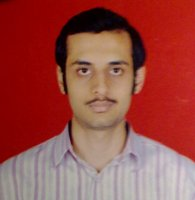
\includegraphics[width=100pt]{gaurav}
    \caption*{Gaurav Dhage\\gr8dhage@gmail.com}
  \end{subfigure}
  \begin{subfigure}[b]{0.24\textwidth}
    \centering
    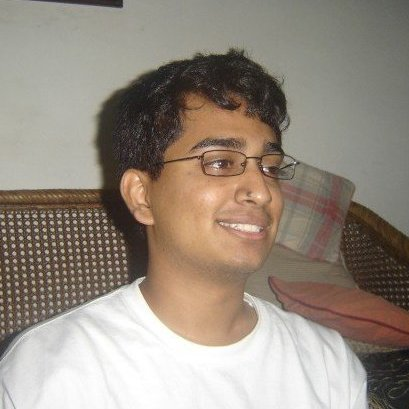
\includegraphics[width=100pt]{anshul}
    \caption*{Anshul Bhatnagar\\anshul.bhatnagar@gatech.edu}
  \end{subfigure}
  \begin{subfigure}[b]{0.24\textwidth}
    \centering
    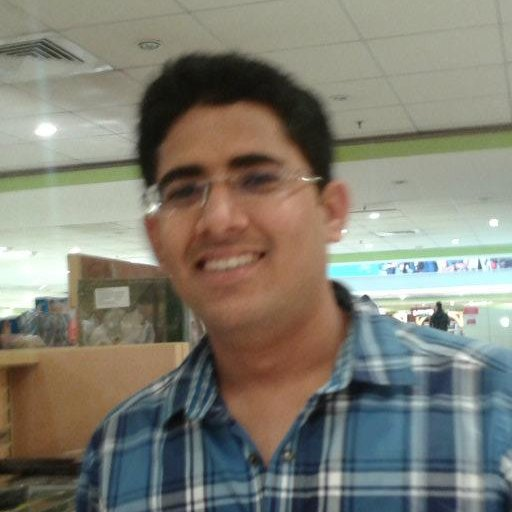
\includegraphics[width=100pt]{suraj}
    \caption*{Suraj Sirpilli@gatech.edu\\surajsirpilli@gatech.edu}
  \end{subfigure}
  \begin{subfigure}[b]{0.24\textwidth}
    \centering
    
\includegraphics[width=100pt]{chris}
    \caption*{Chris Martin\\chris.martin@gatech.edu}
  \end{subfigure}
\end{figure}

\section{Abstract}

The aim of this project is to create a two-player game in which
each player moves disks with the goal of packing them into the
smallest possible circle.

\section{Progress}

\begin{wrapfigure}{r}{0.5\textwidth}
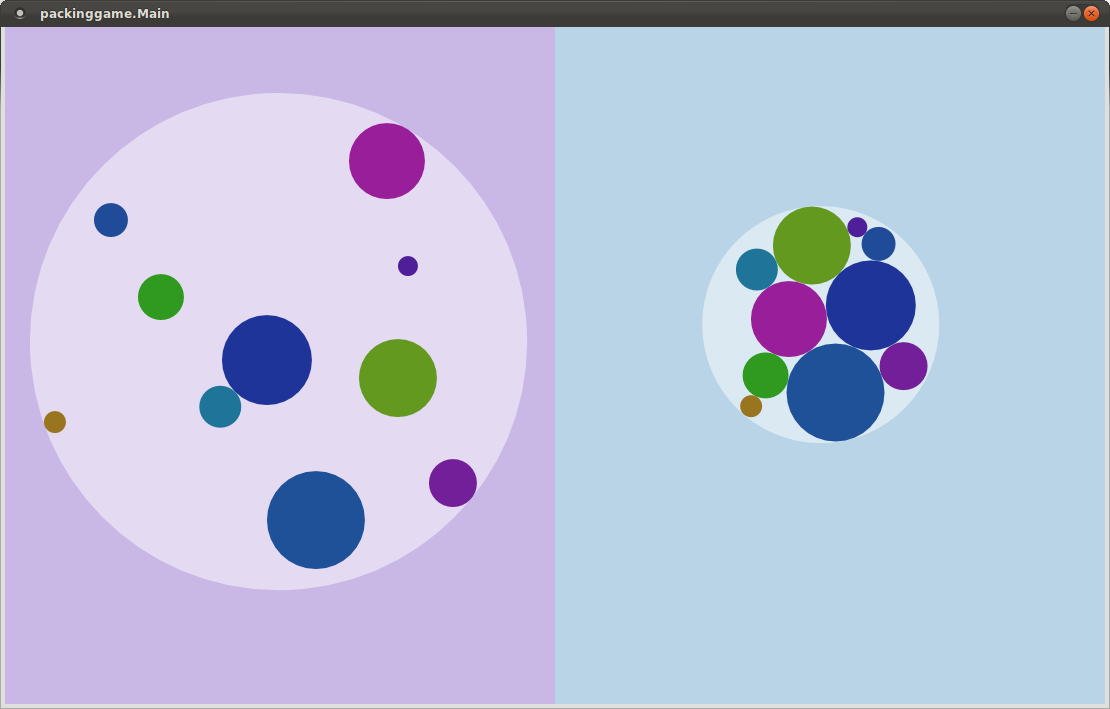
\includegraphics[scale=0.25]{screenshot.png}
\end{wrapfigure}

This phase of the project exhibits the ability to drag disks
using the mouse with collision detection, and compute the
minimal enclosing disk around them.

\section{Collision detection}

When a disk is being moved, we model the situation as a point
being moved among disks that are expanded by the radius of the
moving disk.
If the point intersects a single expanded disk, then we first
try to position the moving disk at the edge of the disk that
overlaps.
If that position overlaps some other disk, then the closest
position for the point is at an intersection of two expanded disks.
We simply choose the closest among all of the $O(n^2)$ intersection points.

\section{Minimal enclosing disk}

Given a fixed center point $c$, we calculate the minimum enclosing radius
as $\max \Big( \textrm{radius}(d) + \textrm{dist}(c, \textrm{center}(d)) \Big)$
over all disks $d$.

The optimal center point is approximated using a random walk.
For a fixed number of iterations, we generate a random vector,
and use it to shift the center if it results in an improvement.

\section{References}

\begin{itemize}

\item Bourke, Paul. {\it Intersection of two circles}.
\url{http://paulbourke.net/geometry/2circle/}

\end{itemize}

\end{document}

